\chapter{Architecture}
\label{ch:architecture}

Now that we already know how to match (by comparing and calculating
\emph{similarity score} from section \ref{ch:nma}), we then proceed
to a bigger picture. This section describes how the architecture
of overall system is.

\section{Initial idea}
\label{sec:initialidea}

Let us start by the basic idea of this project.

As mentioned in section \ref{sec:obj}, the objective of this project is
to provide a web service that produces matching result between two
\emph{lists} of names. As we see the word \emph{list} here, that means
our inputs are not only a pair of names, but rather two lists.
In real world use, this list can be large, a hundred or thousand,
depending on the client who uses the system.

We will introduce two terms, \emph{base name} and \emph{to-match name}.
\emph{Base name} acts as a base and will be matched against each
\emph{to-match name} in their list, from start until the end, then
proceed to the next \emph{base name}, match against the whole
\emph{to-match name} list again, and so on.

\begin{figure}[H]
\centering
\captionsetup{justification=centering}
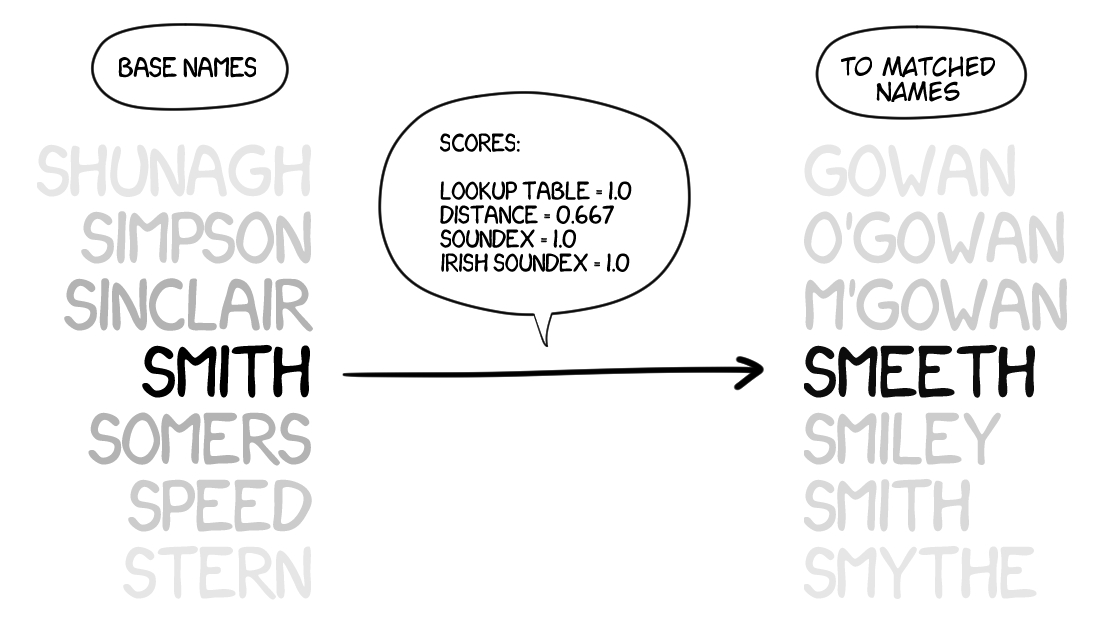
\includegraphics[width=11cm]{gfx/base_tmn}
\caption[\emph{Base name} `SMITH' comparing to \emph{to-match name} `SMEETH'.]{\emph{Base name}
`SMITH' comparing to \emph{to-match name} `SMEETH'. \\
Scores of each matching algorithms
are presented in the bubble above the arrow.}
\label{fig:base_tmn}
\end{figure}

Figure \ref{fig:base_tmn} shows a snapshot of an attempt to match between
\emph{base name} `SMITH' against \emph{to-match name} `SMEETH'.
\emph{Similarity score} for each matching algorithms have been calculated.
And by these scores, we can calculate \emph{overall score} for `SMITH'
and `SMEETH'.

So the next step is to match current \emph{base name}, `SMITH',
against next \emph{to-match name}, `SMILEY'.

Once \emph{base name} `SMITH' completes all \emph{to-match name}\textquotesingle s in their list,
the system then process to the next \emph{base name}, `SOMERS', and start over
the matching process against the whole \emph{to-match name} list again, from
start to the end.

\section{Weighting matching algorithms}
\label{sec:weight}

We realised that, for matching names, each matching algorithms
should not be treated as all the same priority. For example, for Irish names,
it would be better if we favour \emph{Irish soundex} over the
traditional \emph{Soundex}, because it produces more accurate result.

By this idea we also implement \emph{weight} for each matching algorithm.
We will suggest initial values, but also allow client to change these values.
Table \ref{table:weights} states these suggested initial weights.

\begin{table}[H]
  \myfloatalign
  \setlength{\tabcolsep}{0.3cm}
  \begin{tabular}{c c}
    \toprule
    \tableheadline{Matching algorithm} & \tableheadline{Weight} \\
    \midrule
    Levenshtein distance & 1 \\
    Soundex & 3 \\
    Irish soundex & 6 \\
    Lookup table & 10 \\
    \bottomrule
  \end{tabular}
  \caption{Matching algorithm weights.}
  \label{table:weights}
\end{table}

By summarising products of each matching algorithm \emph{similarity score}
and its weight, dividing by sum of all weight, we can obtain
\emph{overall weighted score} (OWS). This sentence can be represented
by equation \ref{eq:ows}.

\begin{equation}
  \begin{gathered}
    OWS = \frac{
      \displaystyle\sum_{i=1}^{n} (s_i \times w_i)
    }{
      \displaystyle\sum_{i=1}^{n} w_i
    }
  \end{gathered}
  \label{eq:ows}
\end{equation}

Where $s$ and $w$ are \emph{similarity score} and weight of
matching algorithm $i$ respectively. $n$ is number of available
matching algorithms.

This \emph{overall weighted score} will represent
each matching and all results will be sorted by this score.
Usage and calculation of this weighting will be described in more detail
in the next section (\ref{sec:actualsys}).

\section{Actual system}
\label{sec:actualsys}

Following our basic idea from previous sections, we then design the
architecture of our system.

Suppose we have two inputs, list of \emph{base names} of length $b$,
and list of \emph{to-match names} of length $t$. We need to
process the matching for $b \times t$ times. We call this single
matching between \emph{base name} and \emph{to-match name}
as \emph{matching cycle}.

In this following figure \ref{fig:overall} we once again show a snapshot
of an attempt to match between \emph{base name} `SMITH'
against \emph{to-match name} `SMEETH'. But now in a \emph{matching cycle} style.

\begin{figure}[H]
\centering
\captionsetup{justification=centering}
\makebox[\textwidth][c]{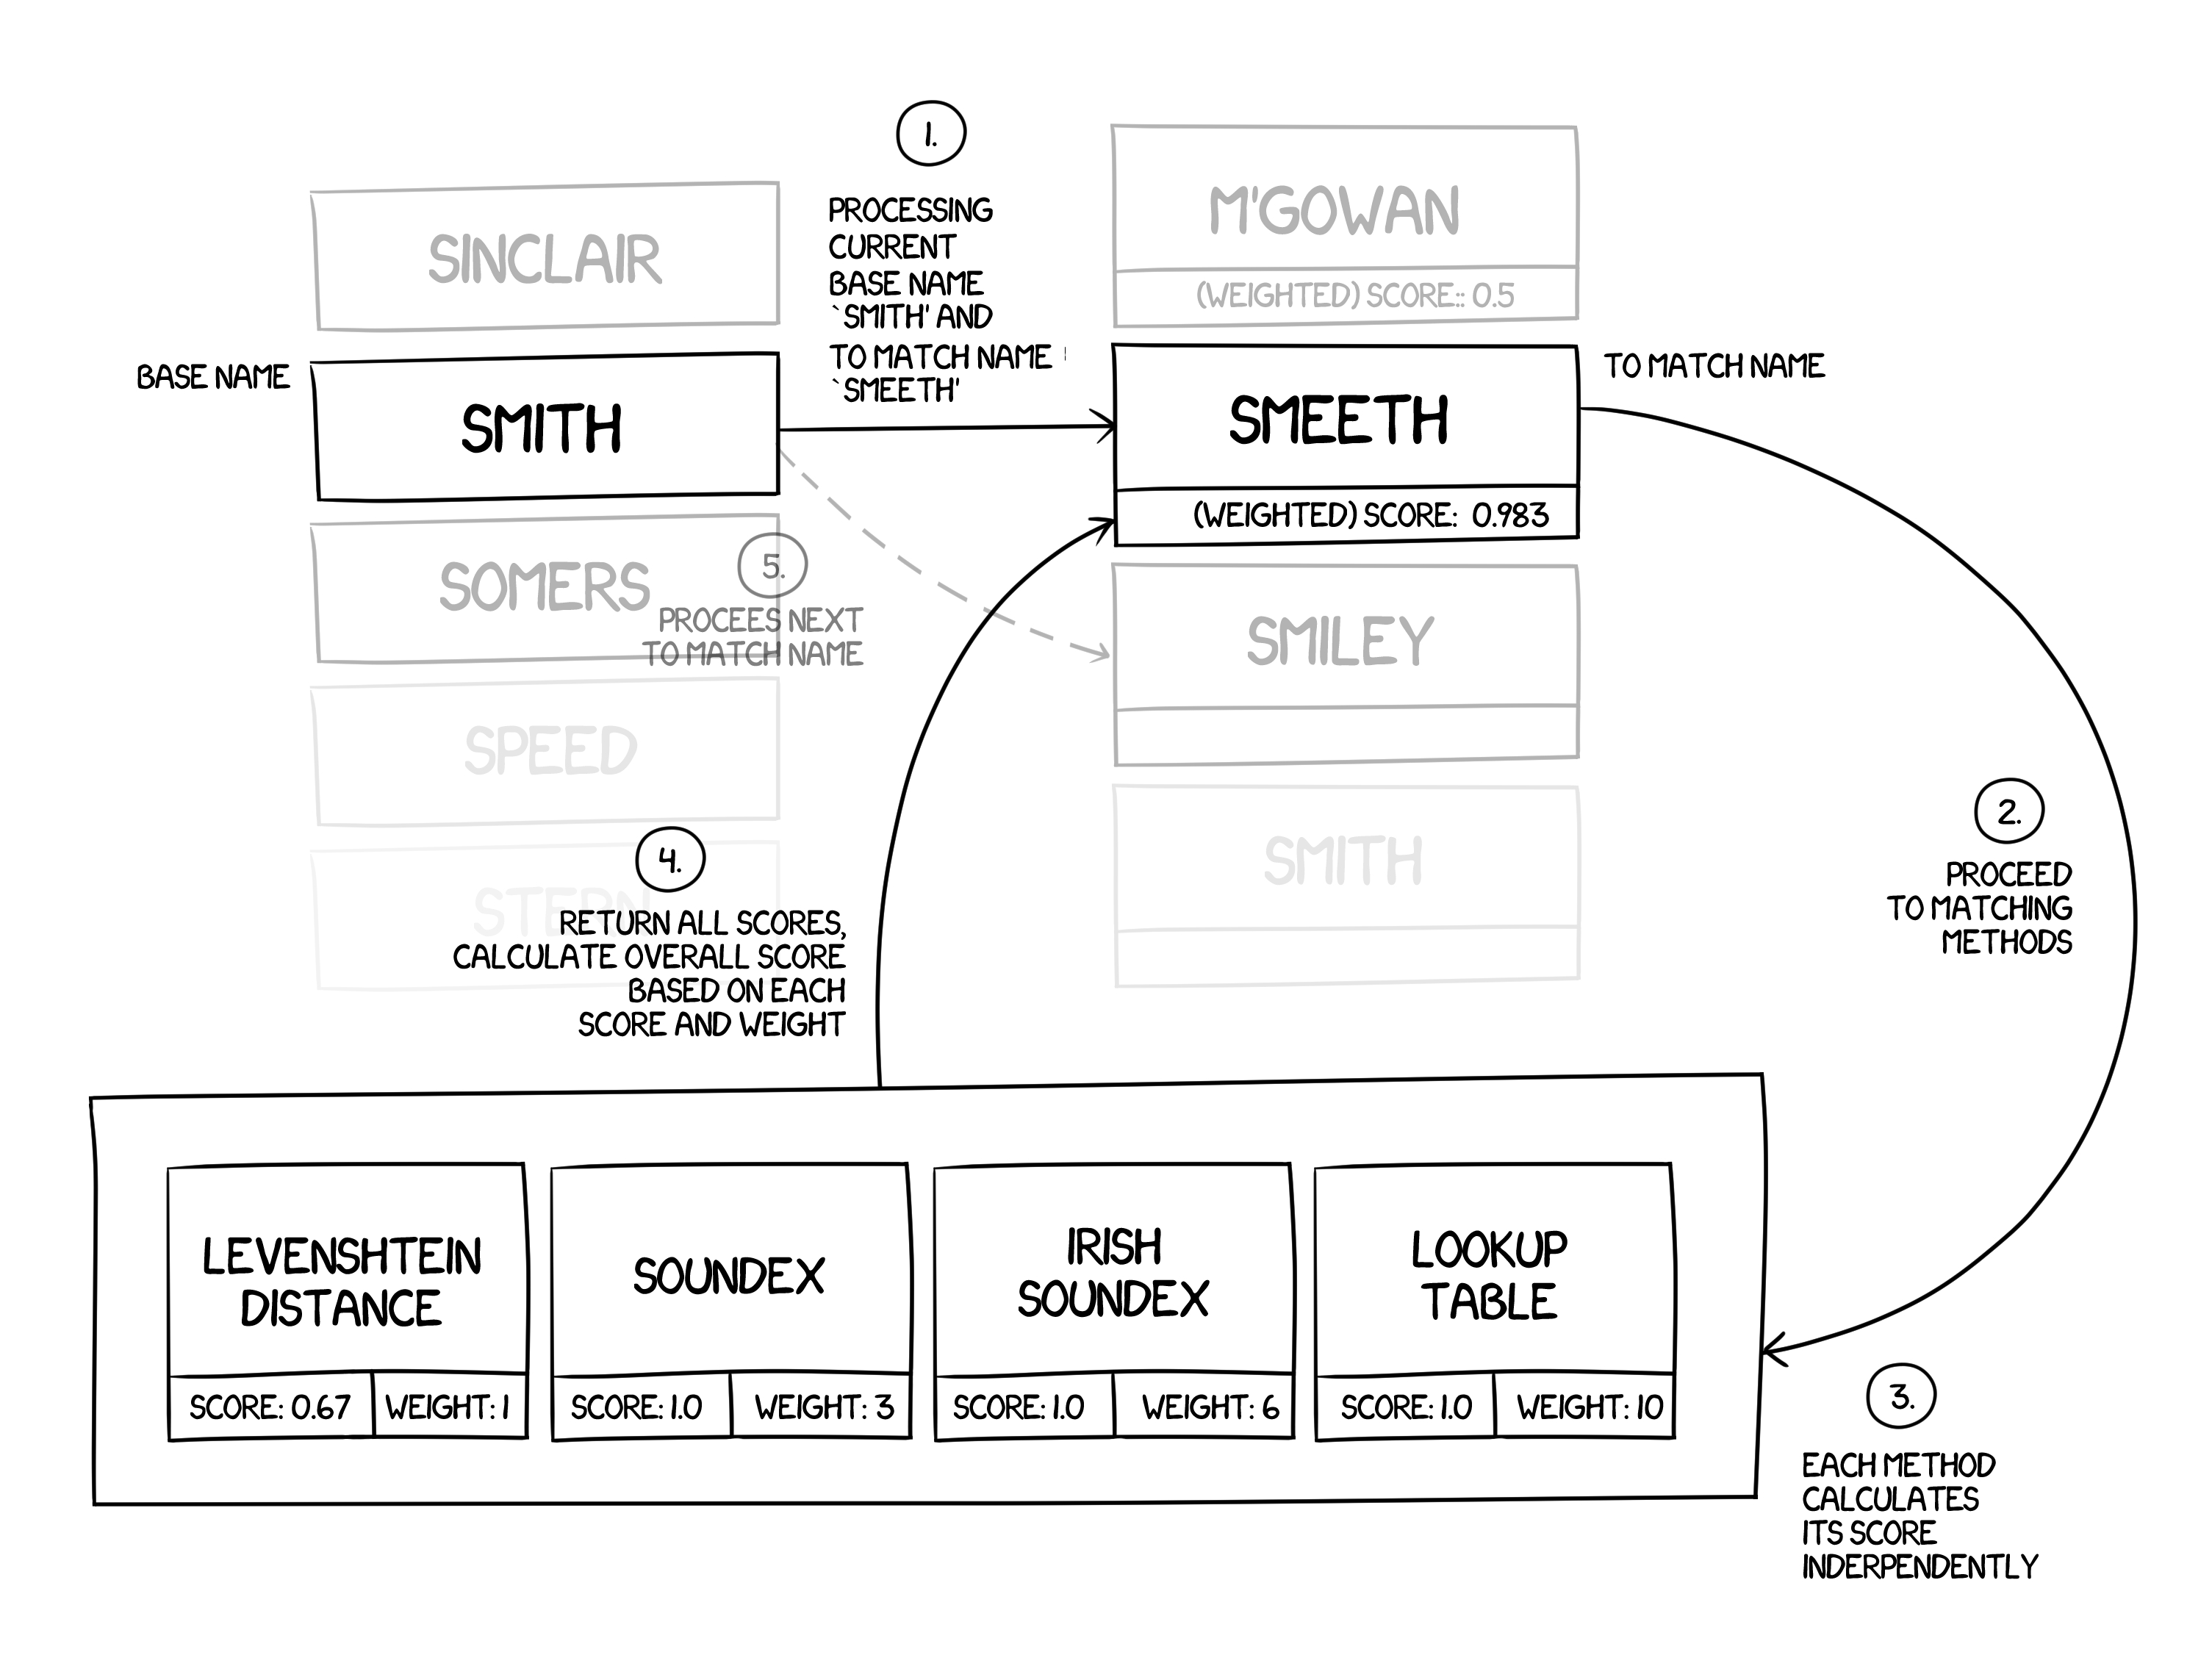
\includegraphics[width=18cm]{gfx/overall}}
\caption{One matching cycle.}
\label{fig:overall}
\end{figure}

One matching cycle consists of 5 steps as shown in figure \ref{fig:overall}.

\begin{enumerate}
  \item Processing current \emph{base name} `SMITH' and \emph{to-match name} `SMEETH'
  \item Proceed to matching algorithms.
  \item Each algorithm calculates its score indepedently.
    \begin{enumerate}
      \item Levenshtein distance between `SMITH' and `SMEETH' is 2
        (1 substitution of \emph{I} to \emph{E} and 1 insertion of \emph{E}).
        So \emph{similarity score} is $(6 - 2) \div 6 = 0.667$ where 6 comes from thelength of the
        longer string, \emph{SMEETH}.

        Weight of this algorithm is 1.

        \textsc{$\therefore$ weighted score = $0.667 \times 1 = 0.667$}
      \item Soundex of both `SMITH' and `SMEETH' are \texttt{S530} so their
        \emph{similarity score} is 1.0.

        Weight of this algorithm is 3.

        \textsc{$\therefore$ weighted score = $1.0 \times 3 = 3.0$}
      \item Irish soundex of both `SMITH' and `SMEETH' are \texttt{S530} so their
        \emph{similarity score} is 1.0.

        Weight of this algorithm is 6.

        \textsc{$\therefore$ weighted score = $1.0 \times 6 = 6.0$}
      \item References between `SMITH' and `SMEETH' is found in the
        Lookup table via group 1897. so their \emph{similarity score} is 1.0

        Weight of this algorithm is 10.

        \textsc{$\therefore$ weighted score = $1.0 \times 10 = 10.0$}
    \end{enumerate}
  \item Return all scores and then calculate \emph{overall weighted score}
    for `SMITH' and `SMEETH'. Sum of the scores is
    $0.667 + 3.0 + 6.0 + 10.0 = 19.667$. Sum of the weights is
    $1 + 3 + 6 + 10 = 20$. Therefore the \emph{overall weighted score} is
    $19.667 \div 20 = 0.983$.
  \item Matching cycle for `SMITH' and `SMEETH' is finished with
    \emph{overall weighted score} 0.983.
    Now the system will proceed to the next \emph{to-match name} `SMILEY'.
    Matching cycles for \emph{base name} `SMITH' will continue until
    the end of \emph{to-match name} list. After that it will start
    matching cycles for \emph{base name} `SOMERS' from the start of
    \emph{to-match names}, and so on.
\end{enumerate}

Once all cycles are fully finished for every \emph{base names} and
\emph{to-match names}, we will get all \emph{overall weighted scores}
ready. So we can sort and present in web interface (section \ref{sec:wi}), or return
as a result in web service (section \ref{sec:ws}).

\section{Thresholding the results}
\label{sec:threshold}

Suppose there are a thousand of \emph{to-match names}, there could be
many irreverent results that are not likely to match each
\emph{base name}. For example \emph{overall weighted scores} of
`SMITH' and `CROMBIE' is just 0.007.

Client may opt-out these irreverent results by specifying
a floating number \emph{threshold}.
Any \emph{to-match name} with \emph{overall weighted scores}
lower than \emph{threshold} will be discarded from the result.

\section{Data flow}
\label{sec:mcv}

In the previous section we describe the essence of this project,
how we use matching algorithms to calculate score of similarity
between two strings. We know how to process the data.
Now in order to make the system becomes useable.
We need to consider two more things.

\begin{itemize}
  \item How to gather inputs from clients.
  \item How to present or return results to clients.
\end{itemize}

From research questions (section \ref{sec:rq}) we mentioned
two ways to communicate with clients, by \emph{web service} and
\emph{web interface}.

Clients who use the system as a web service
will send inputs directly without any medium in between, and will
receive result back in form of agreed format, e.g. \texttt{JSON}.

On the other hand, clients who use the system via web interface
will use a form in a web interface (web page) provided by the system to provide
inputs, and results will be presented in another page
after client submitted the form.

\begin{table}[H]
  \myfloatalign
  \setlength{\tabcolsep}{0.3cm}
  \begin{tabular}{l p{4cm} l}
    \toprule
    \tableheadline{Service type} & \tableheadline{Input source} & \tableheadline{Result format}  \\
    \midrule
    Web service & Web/mobile/desktop application & \texttt{JSON} \\
    \midrule
    Web interface & Provided form & Web page result \\
    \bottomrule
  \end{tabular}
  \caption{Service types and their inputs and results.}
  \label{table:dataflow}
\end{table}

In the next section (\ref{sec:mvc}) we will describe how we
gather inputs and provide results.

\section{MVC}
\label{sec:mvc}

Our system is based on Ruby on Rails, which is a MVC\footnote{Model-View-Controller
\cite[]{mvc}} framework. We will use Rails architecture to encapsulate
our system be these following means.

\begin{description}
  \item[View:] where the form for web interface is implemented.
    It creates a web page with inputs for use to fill in.
    Client can inputs names manually, or upload a file
    containing names. He also can choose whether to use any
    available matching algorithms.

    Inputs from \emph{view} are then passed to \emph{controller}.

    \emph{View} is also responsible in displaying result to
    web interface clients, and generating \texttt{JSON} result
    for web service clients.
  \item[Controller:] receives inputs from different sources,
    inputs from form of web interface style, or direct input from clients
    using web service style. Inputs will be pre-processed, such as
    separating lines from file input, removing white spaces,
    or converting input to upper-case.

    Once inputs are ready, \emph{controller} then passes these inputs
    to \emph{model}, where our matching system lies in.

    After inputs are processed, \emph{controller} receives results
    back from \emph{model}, then \emph{controller} will decide
    which kind of result it needs to return from input source.
    It will then pass results to appropriate \emph{view}.
  \item[Model:] this is where we implement our whole matching system in.
    Model constructs \emph{base names} and \emph{to-match names}
    from received inputs, then invoke matching algorithms, as described
    in section \ref{sec:actualsys}. \emph{Model} will pass results back to
    \emph{controller} after finished.
\end{description}

\begin{figure}[H]
\centering
\captionsetup{justification=centering}
\makebox[\textwidth][c]{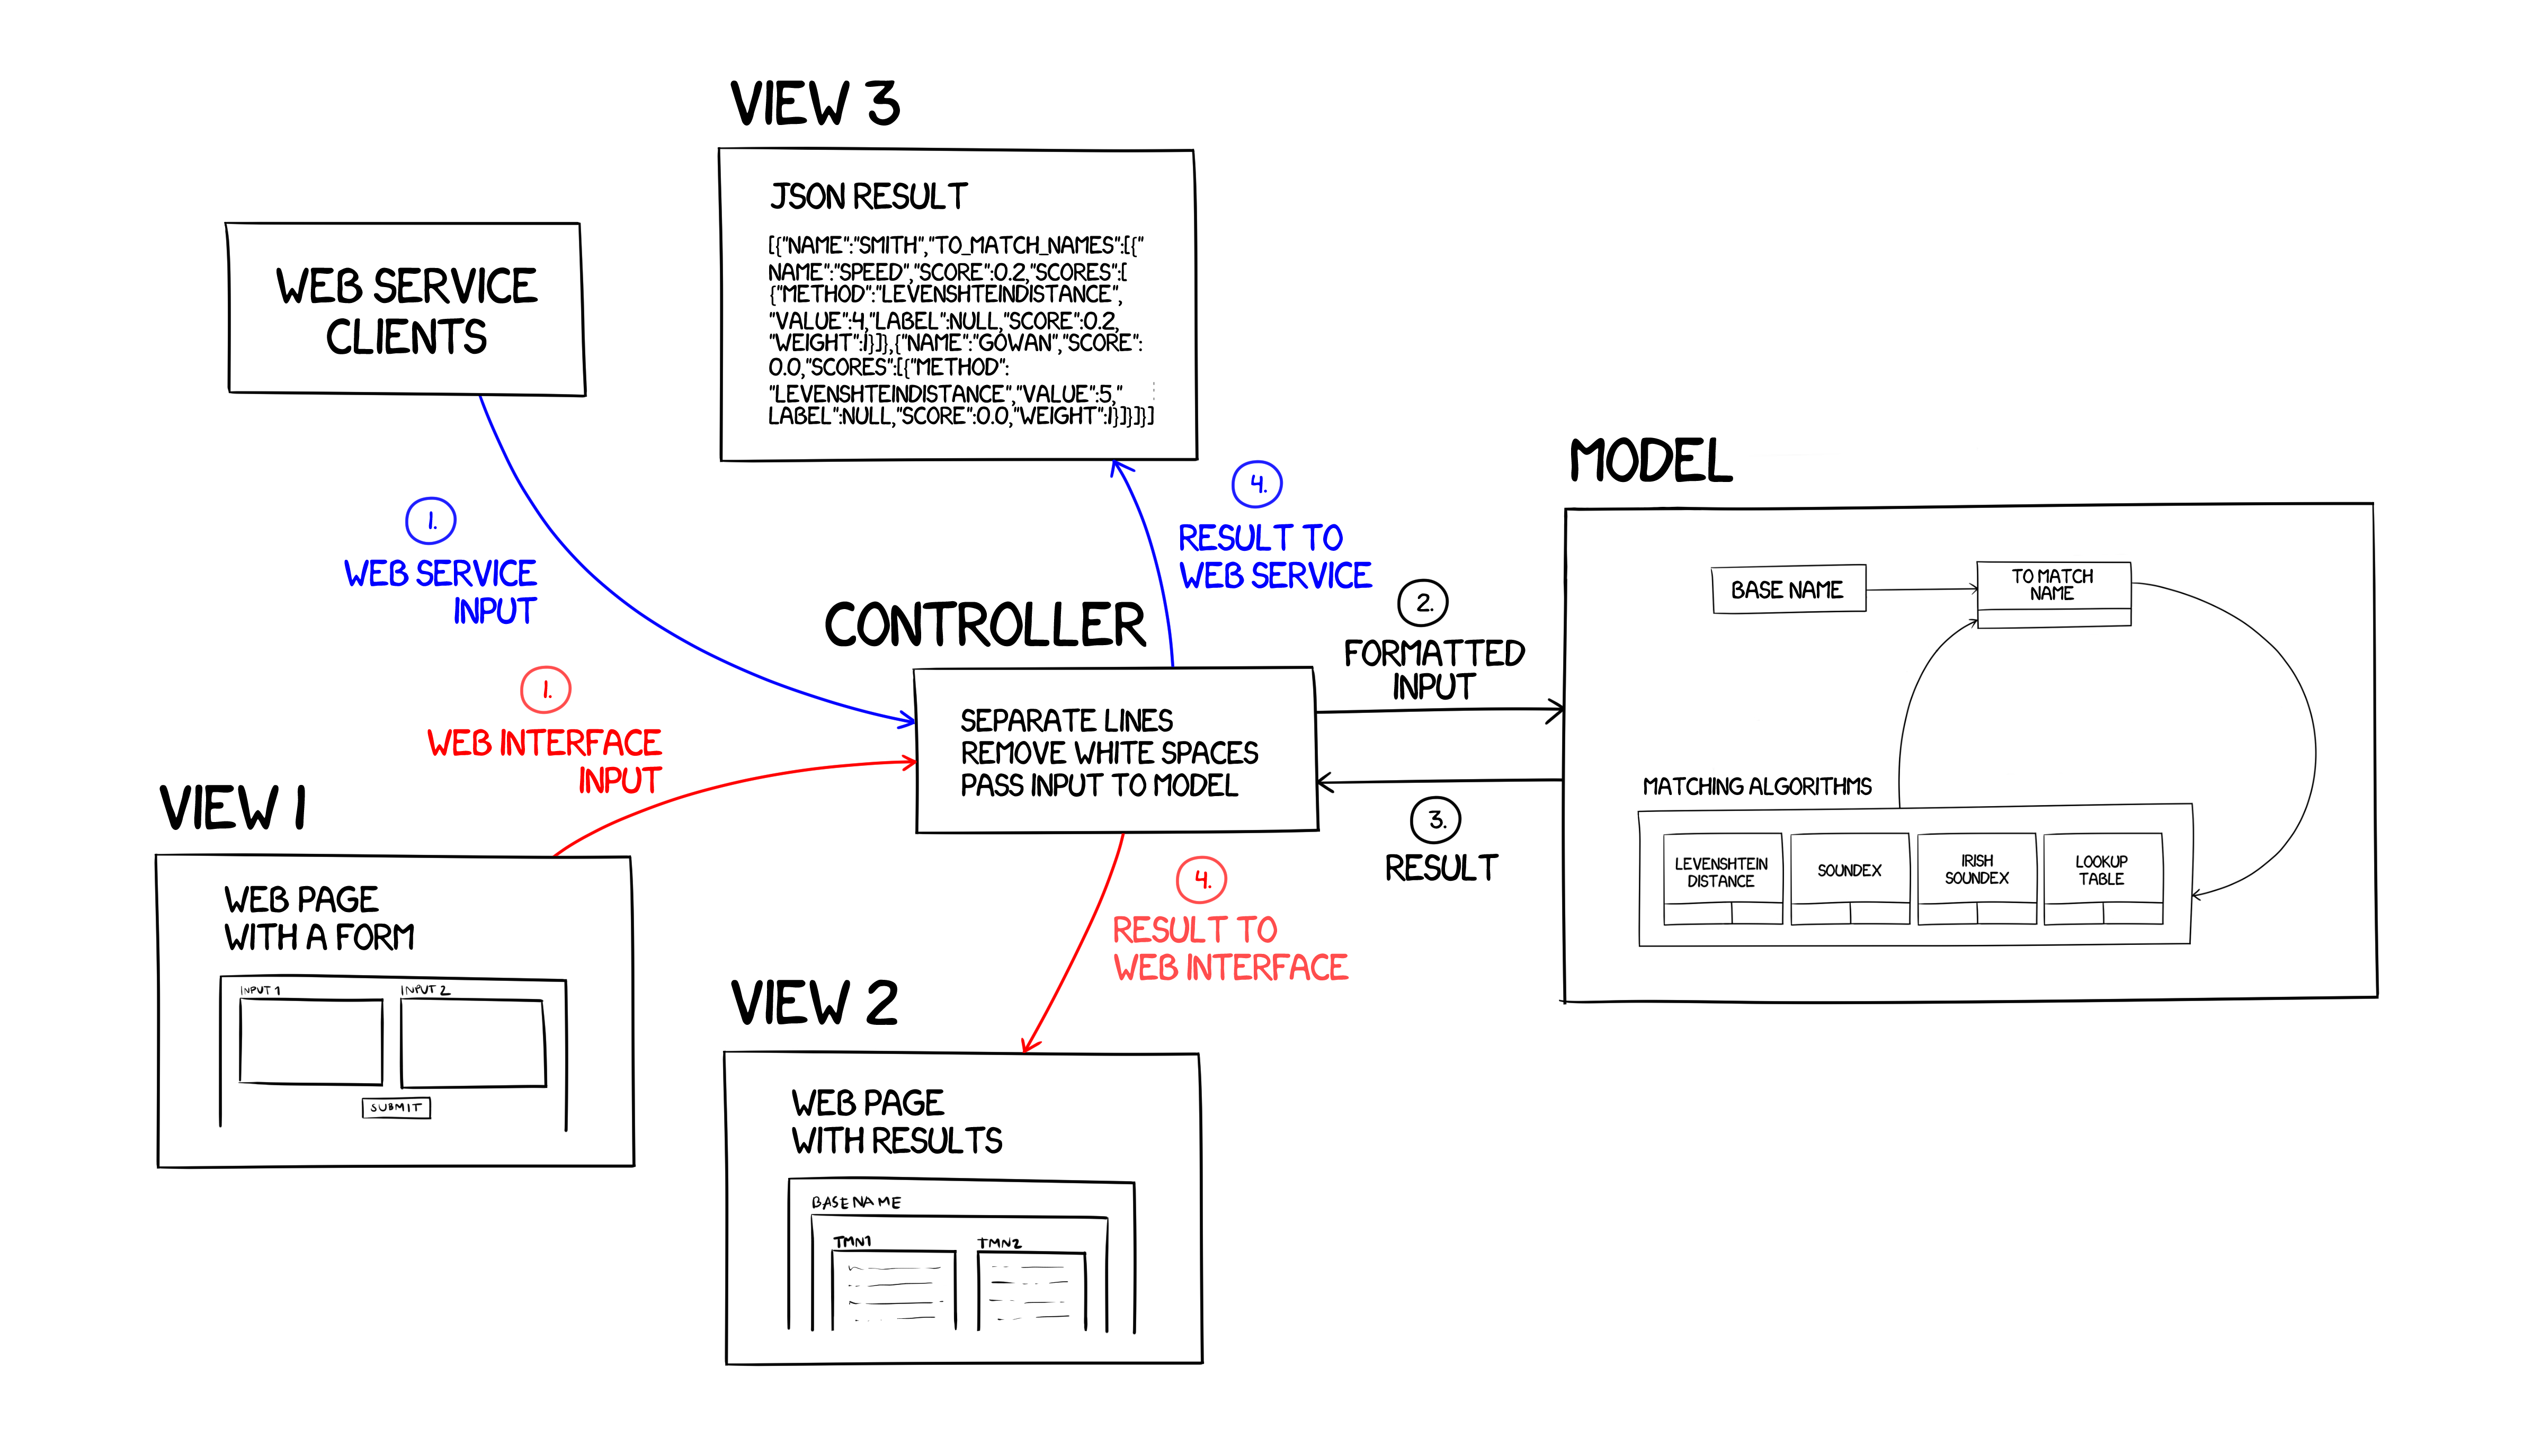
\includegraphics[width=18cm]{gfx/mvc}}
\caption{Data flow from web service client and web interface client.}
\label{fig:mvc}
\end{figure}

\section{Web Service}
\label{sec:ws}

From figure \ref{fig:mvc}, web service clients use the system
by directly pass inputs to the \emph{controller}. Recalling
from previous sessions, all possible inputs to the system
are as follow.

\begin{enumerate}
  \item Base names -- separated by
        new lines\footnote{\texttt{Preferably \textbackslash n} or \texttt{\textbackslash r}, see \url{http://stackoverflow.com/questions/1761051/difference-between-n-and-r}.}.
  \item To-match names -- separated by new lines.
  \item Matching algorithms -- specify needed algorithm names along with its weight (section \ref{sec:weight}).
  \item Threshold (section \ref{sec:threshold}).
  \item Standard list -- will be introduced in section \ref{sec:stdname}.
    Specify \texttt{true}, \texttt{t}, or \texttt{1} to use the standard list.
\end{enumerate}

Currently a preferable format is \texttt{JSON}. In listing \ref{lst:json}
shown a sample \texttt{JSON} input for using web service, let us
call this \texttt{sample.json}.

\begin{minipage}{\linewidth}
\begin{lstlisting}[language={json}, label={lst:json}, caption={\texttt{sample.json}.}]
{
  "base_names":"Smith",
  "to_match_names":"Smythe\r\nO'Gowan",
  "matching_algorithms":{
    "1":{"name":"LookupTable", "weight":"10"},
    "2":{"name":"LevenshteinDistance", "weight":"1"},
    "3":{"name":"Soundex", "weight":"3"},
    "4":{"name":"IrishSoundex", "weight":"6"}
  },
  "threshold":"0",
  "standard_list":""
}
\end{lstlisting}
\end{minipage}

\texttt{sample.json} is an attempt to match between \emph{base name} `SMITH',
and \emph{to-match name} `SMYTHE' and `O\textquotesingle GOWAN'. Using 4 matching
algorithms, and threshold as 0. We will submit this \texttt{sample.json} input
to the system using cURL \cite[]{curl} in command line.

\begin{minipage}{\linewidth}
  \begin{lstlisting}[language={bash}, label={lst:curl}, caption={}]
$ curl -H "Accept: application/json" -H "Content-type: application/json" -X POST -d @sample.json http://localhost:4001/match.json
\end{lstlisting}
\end{minipage}

We use HTTP POST \cite[]{post} to submit \texttt{sample.json} to the web service,
currently running locally, so the \texttt{url} using here is \url{http://localhost:4001/match.json}.
The formatted \texttt{JSON} result is shown in listing \ref{lst:curl2},
note that the result of matching between `SMITH' and `O\textquotesingle GOWAN' is truncated
just for readability.

\begin{lstlisting}[language={json}, label={lst:curl2}, caption={Result from \texttt{sample.json}.}]
[
  {
    "base_name": "SMITH",
    "to_match_names": [
      {
        "to_match_name": "SMYTHE",
        "overall_weighted_score": 0.983,
        "scores": [
          {
            "method": "LookupTable",
            "value": "Matched",
            "label": "1897",
            "score": 1,
            "weight": 10
          },
          {
            "method": "LevenshteinDistance",
            "value": 2,
            "label": null,
            "score": 0.667,
            "weight": 1
          },
          {
            "method": "Soundex",
            "value": "S530 <=> S530",
            "label": null,
            "score": 1,
            "weight": 3
          },
          {
            "method": "IrishSoundex",
            "value": "S530 <=> S530",
            "label": "SMYTHE",
            "score": 1,
            "weight": 6
          }
        ]
      },
      {
        "to_match_name": "O'GOWAN",
        "overall_weighted_score": 0.5,
        ...
\end{lstlisting}

From the results, \emph{overall weighted score} between `SMITH' and `SMYTHE'
is 0.983, higher than `SMITH' and `O\textquotesingle GOWAN' (0.5), so the former is sorted
before the latter.

To generate these results in \texttt{JSON}, we use Jbuilder \cite[]{jbuiler},
a template for generating JSON structures. The template we use is shown
in listing \ref{lst:jbuilder}.

\begin{minipage}{\linewidth}
\begin{lstlisting}[label={lst:jbuilder}, caption={Jbuilder template for generating \texttt{JSON} results.}]
json.array! @matched_names do |matched_name|
  json.base_name matched_name.name

  json.to_match_names do
    json.array! matched_name.to_match_names do |tmn|
      json.to_match_name tmn.name
      json.overall_weighted_score tmn.score

      json.scores do
        json.array! tmn.scores do |s|
          json.method s.class.name
          json.value s.value
          json.label s.label
          json.score s.score
          json.weight s.weight
        end
      end
    end
  end
end
\end{lstlisting}
\end{minipage}


\section{Web Interface}
\label{sec:wi}

Our system provides a web interface with inputs form.
All possible inputs are equivalent to web service as follow.

\begin{enumerate}
  \item Base names -- clients can fill the names in \emph{input 1}, separated
    by new lines. alternatively, clients can also upload a file containing names
    separated by new lines. if the web interface detects that the file input
    is present, direct text input will be discarded.
  \item To-match names -- the same way of \emph{base name}, using \emph{Input 2}.
  \item Matching algorithms -- clients can choose available algorithms
    from the list along with its weight using checkboxes. Uncheck to
    opt-out any algorithms.
  \item Threshold -- clients can specify floating number threshold using input box.
  \item Standard list -- will be introduced in section \ref{sec:stdname}.
    clients can check the checkbox to use the standard list.
\end{enumerate}

\begin{figure}[H]
\centering
\captionsetup{justification=centering}
\makebox[\textwidth][c]{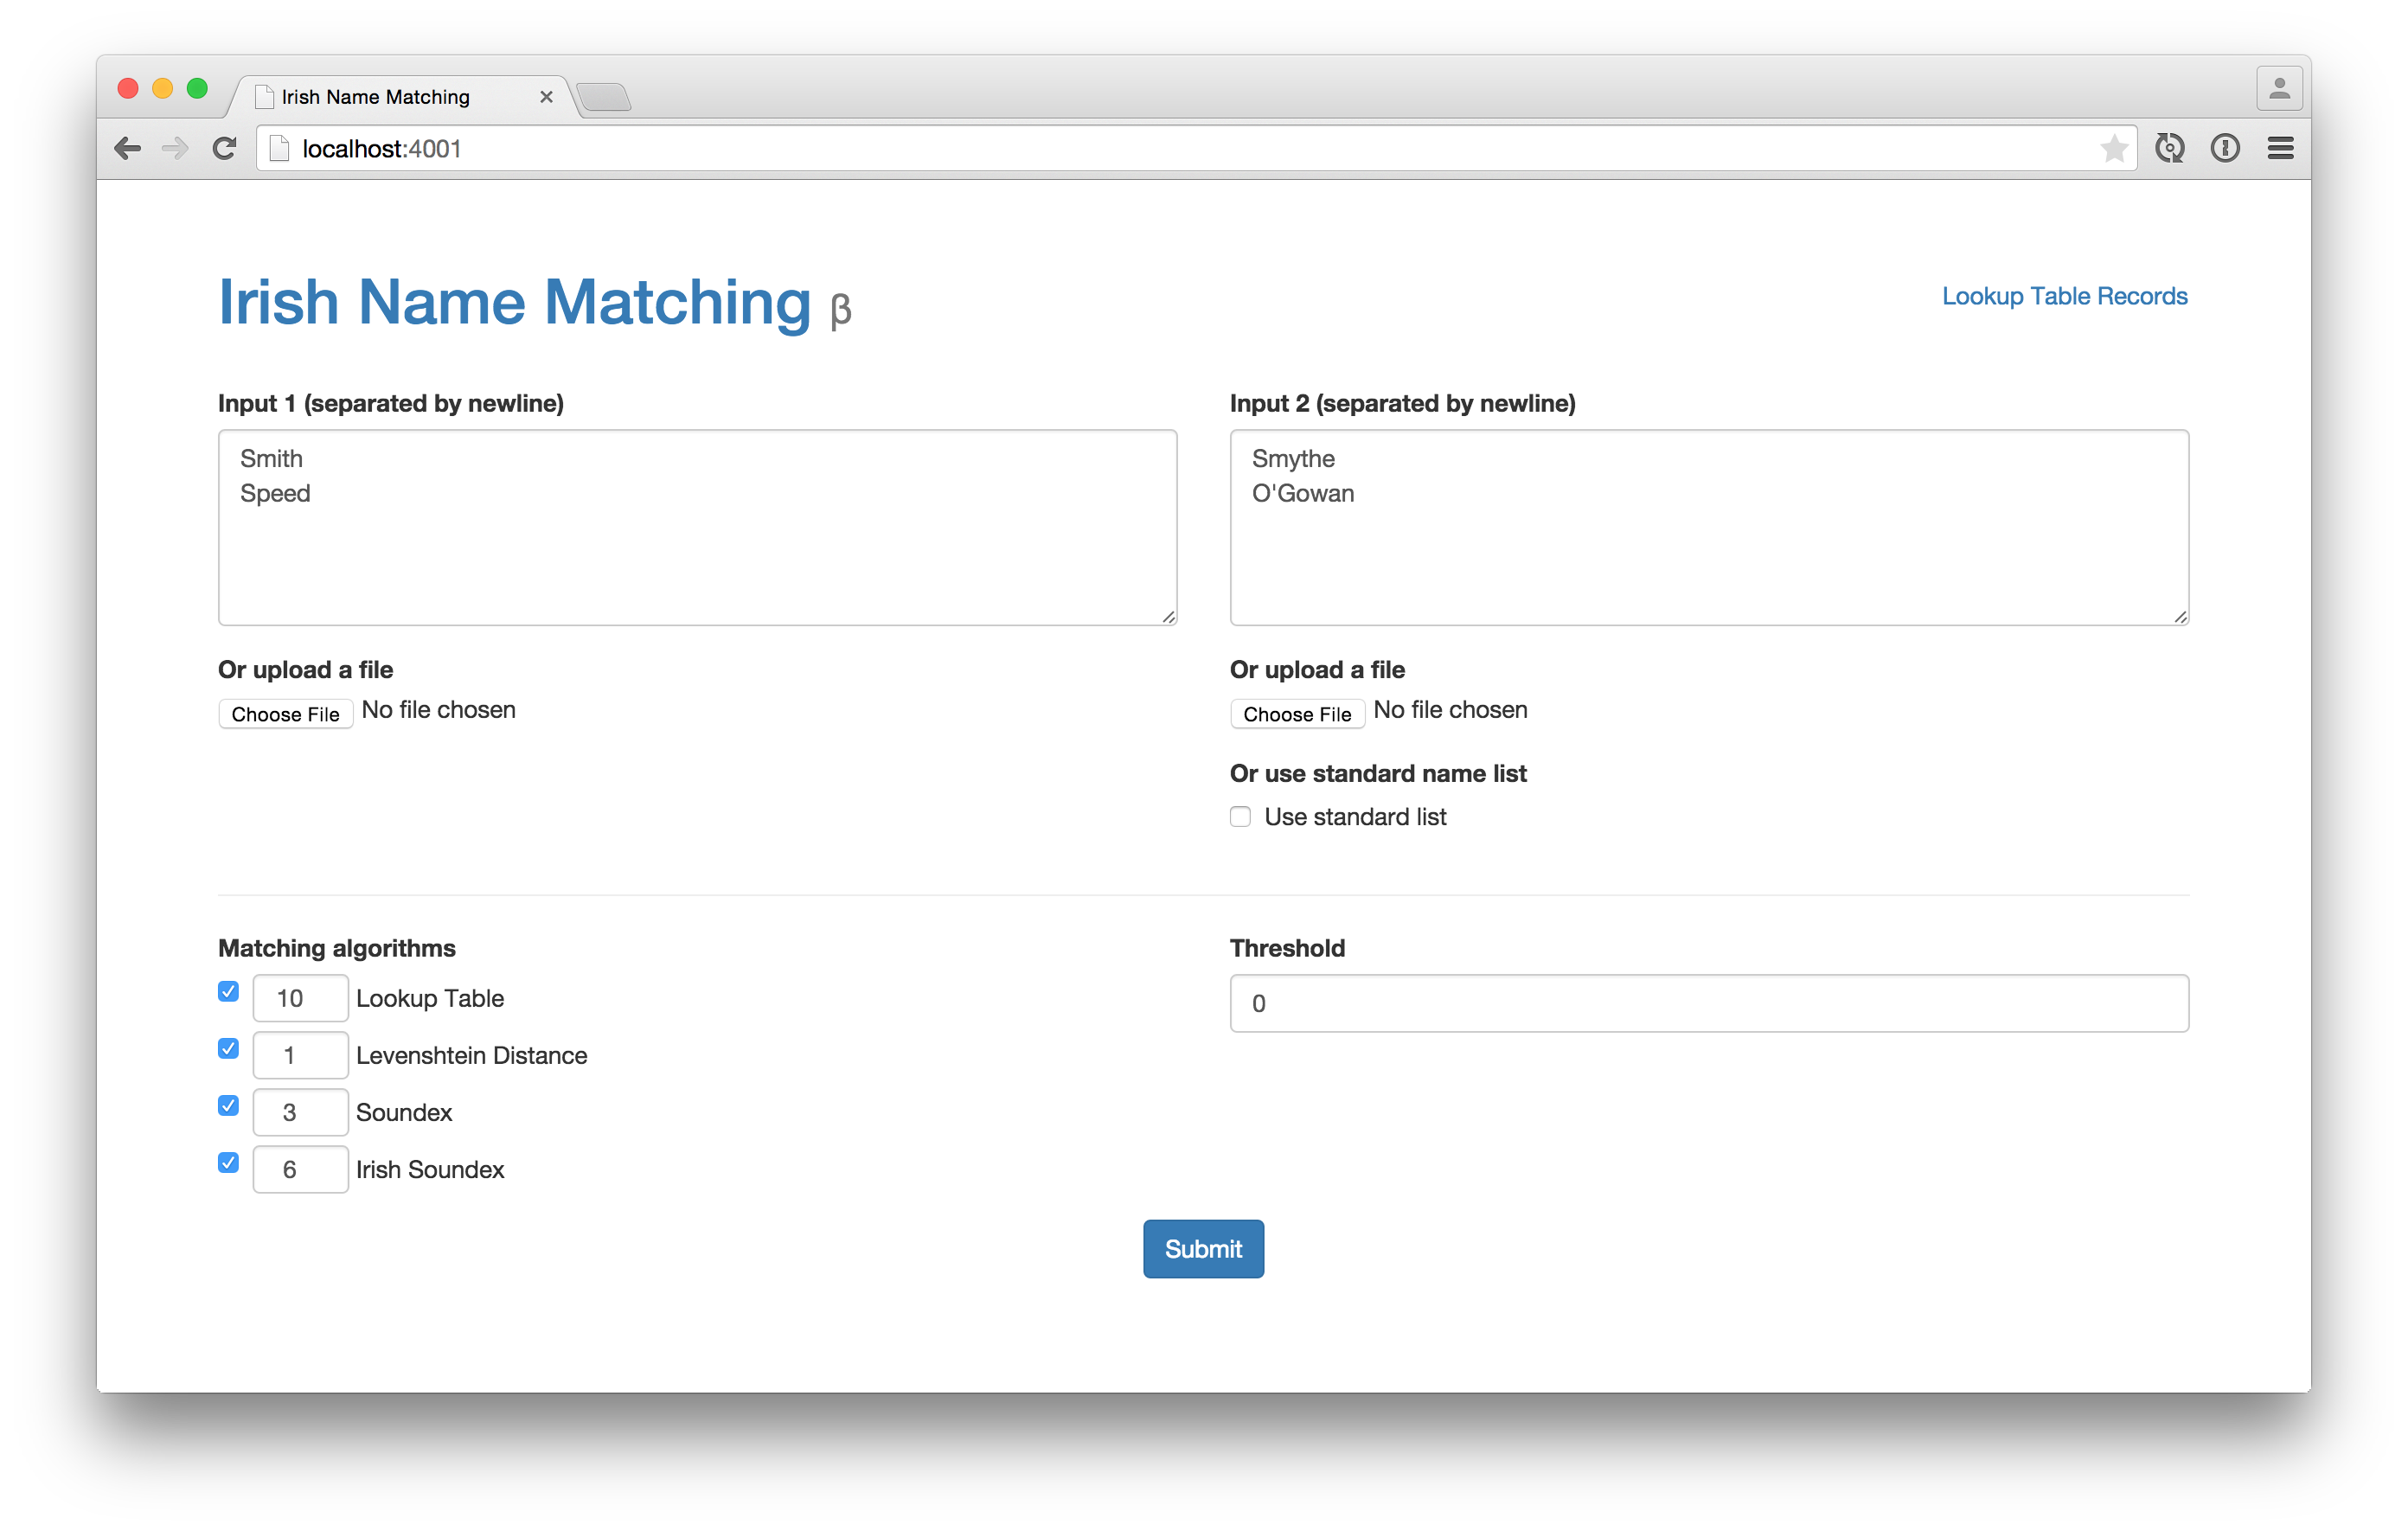
\includegraphics[width=16cm]{gfx/web_interface}}
\caption{Web interface with input forms.}
\label{fig:wi}
\end{figure}

Figure \ref{fig:wi} is an attempt to match between \emph{base name} `SMITH'
and `SPEED', and \emph{to-match name} `SMYTHE' and `O\textquotesingle GOWAN'. Using 4 matching
algorithms, and threshold as 0. After finish filling all inputs client
may press the blue `Submit' button to begin matching.

\begin{figure}[H]
\centering
\captionsetup{justification=centering}
\makebox[\textwidth][c]{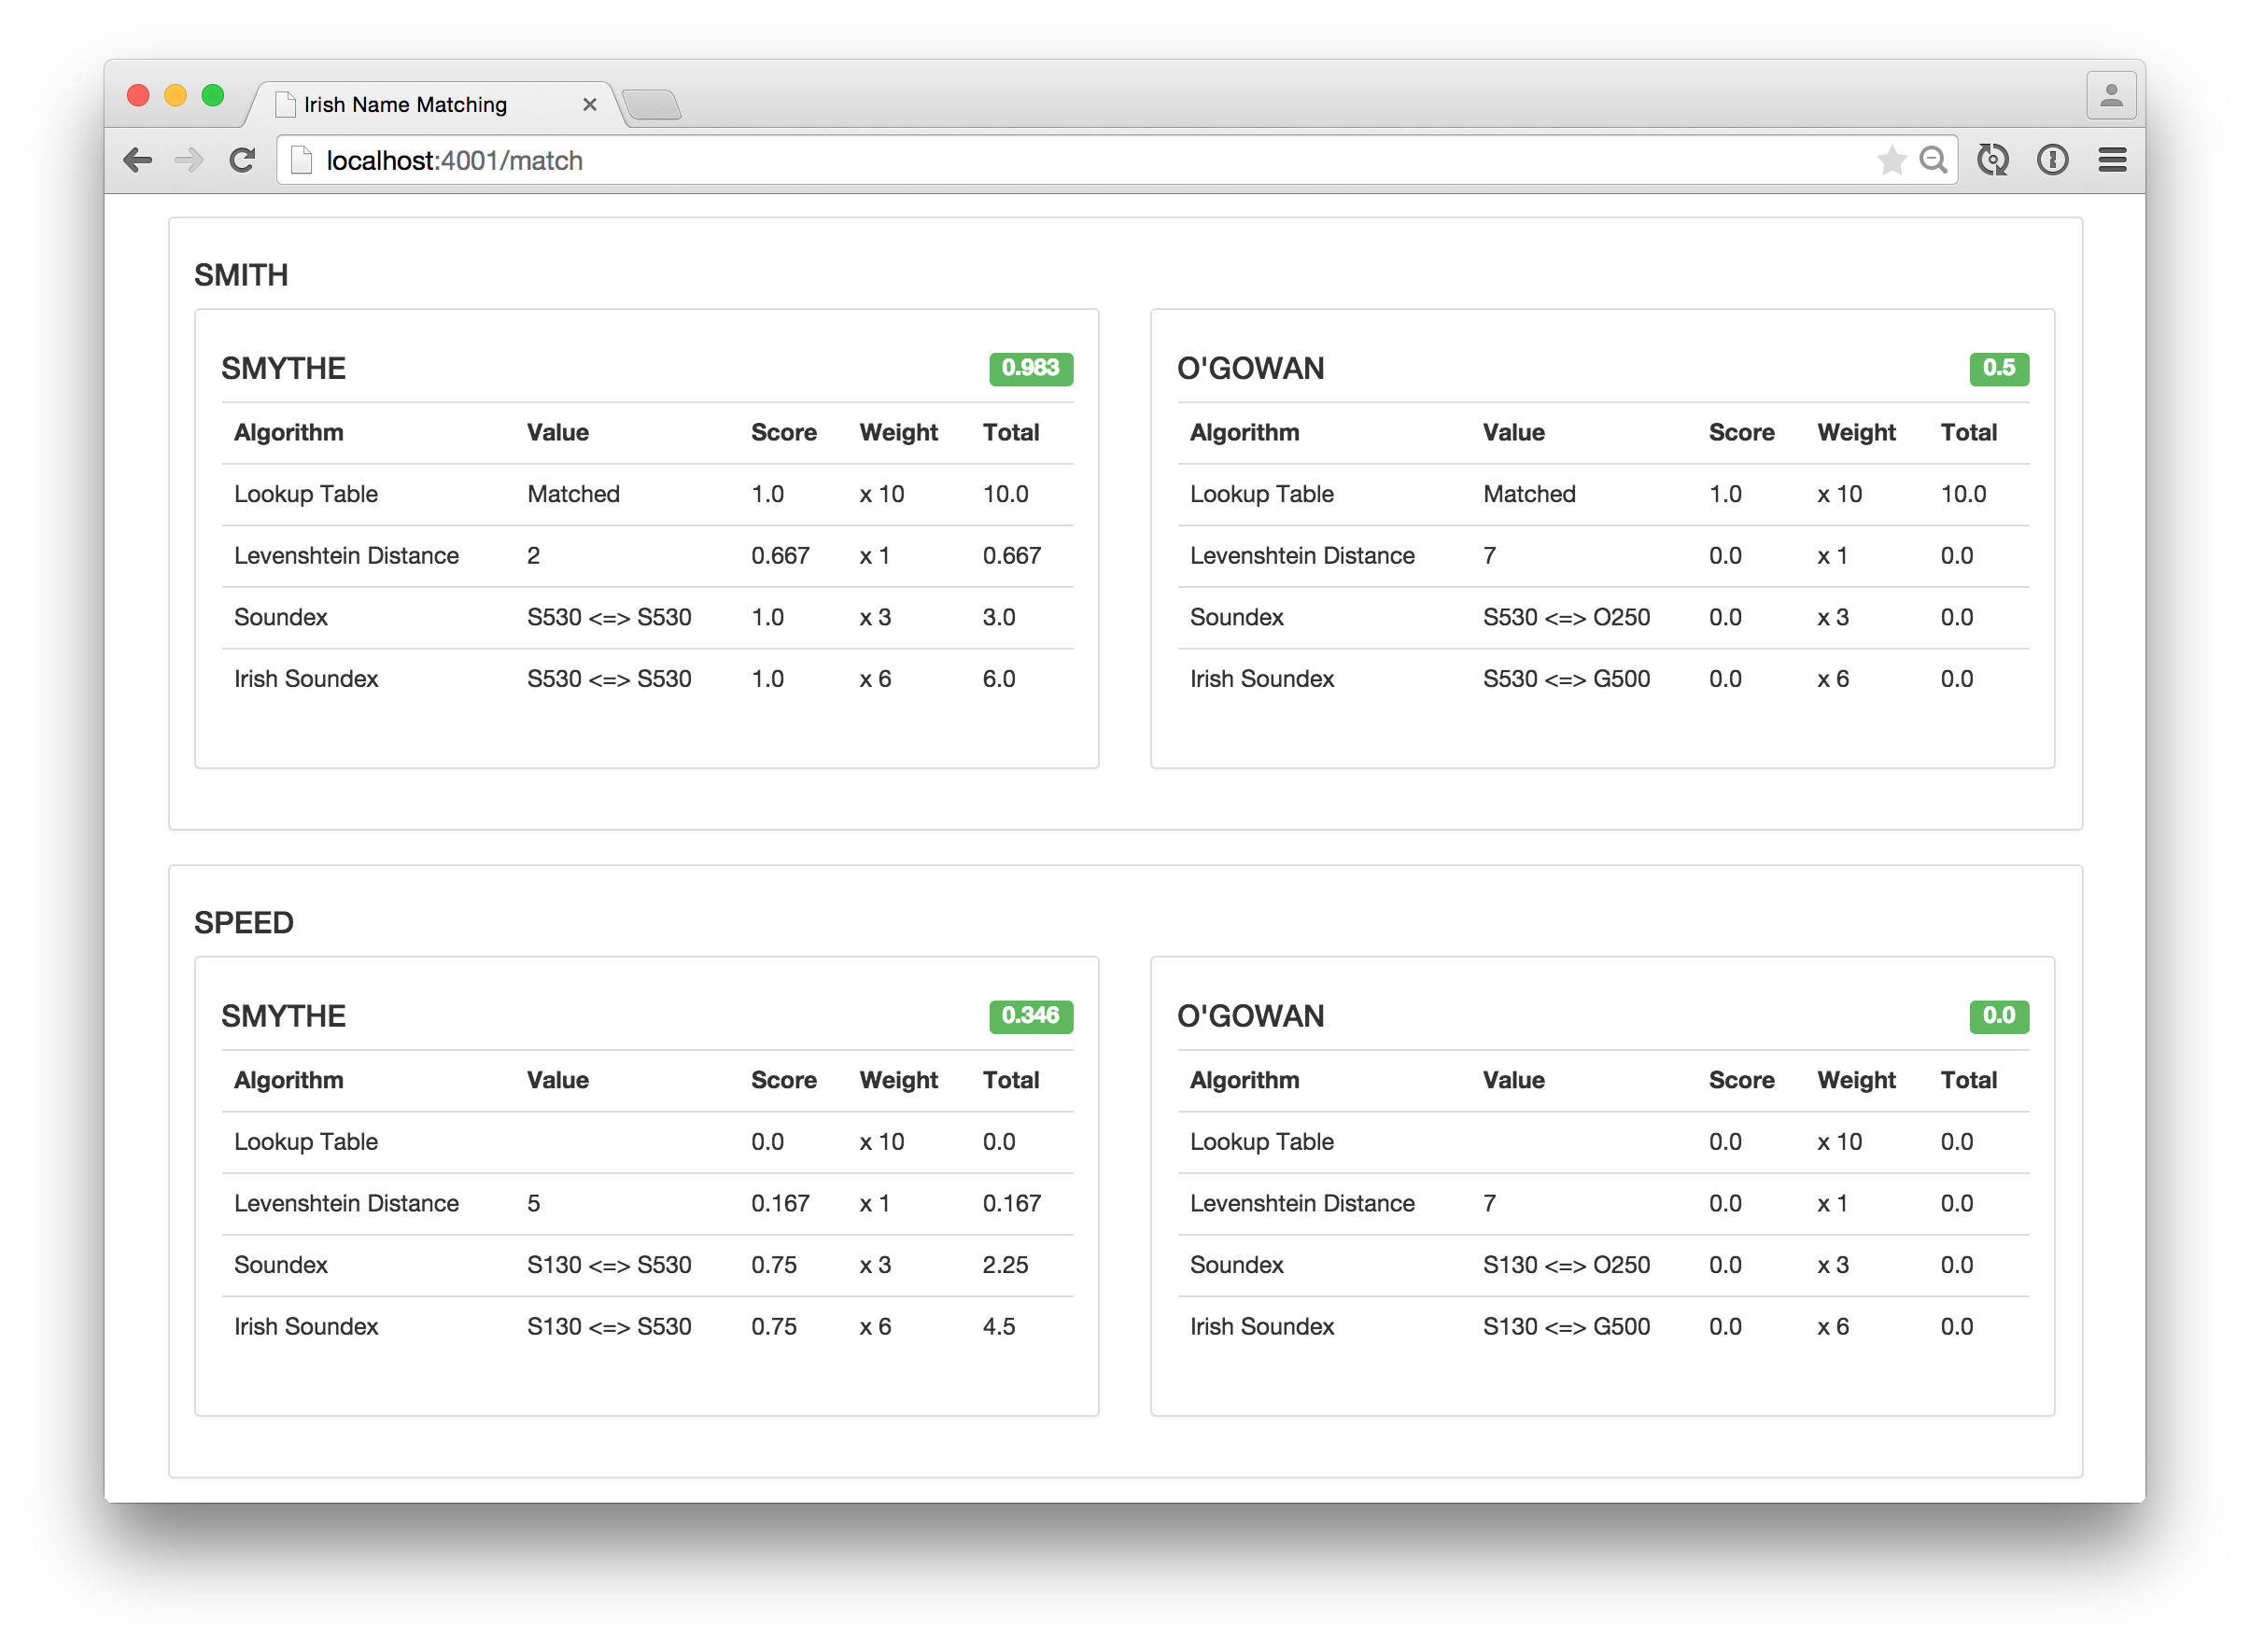
\includegraphics[width=16cm]{gfx/web_interface_result}}
\caption{Web interface results page.}
\label{fig:wi_res}
\end{figure}

Figure \ref{fig:wi_res} shows the web interface result of this matching.
There are two \emph{base names} and two \emph{to-match names}, so the results
are matchings of total $2 \times 2 = 4$ names. Each outer box is results
of matching between each \emph{base names}, with the outer box there
is an inner box containing details of each \emph{to-match names}.

From the results, \emph{overall weighted score}
(each green labelled box) between `SMITH' and `SMYTHE'
is 0.983, higher than `SMITH' and `O\textquotesingle GOWAN' (0.5), so the former is sorted
before the latter.
